\documentclass[11pt]{article}

\usepackage[utf8]{inputenc}
\usepackage[T1]{fontenc}
\usepackage{lmodern}
\usepackage[margin=1in]{geometry}
\usepackage{graphicx}
\usepackage{booktabs}
\usepackage{amsmath}
\usepackage{siunitx}
\usepackage{caption}
\usepackage{subcaption}
\usepackage{float}
\usepackage[hidelinks]{hyperref}
\usepackage[round]{natbib}
\usepackage{xcolor}
\usepackage{enumitem}

\graphicspath{{figures/}}
\captionsetup{font=small,labelfont=bf}
\setlength{\parskip}{0.4em}
\setlength{\parindent}{0pt}

\title{\textbf{Which explanations can we trust? A multi-method faithfulness,
cross-method agreement, and anatomical-validity audit of a frozen pretrained
SFCN on pediatric brain MRI}}

\author{Houssem Eddine\\[2pt]
\small ESPRIT, Tunis, Tunisia\\
\small \texttt{houssemeddineds@gmail.com}\\
\small ORCID: \href{https://orcid.org/0009-0007-2027-2520}{0009-0007-2027-2520}}

\date{}

\begin{document}
\maketitle

\begin{abstract}
\noindent
Explanation methods are routinely used to justify clinical claims from 3D brain-MRI
classifiers, yet they are rarely validated before being believed. We audit nine
attribution methods on a frozen pretrained Simple Fully Convolutional Network (SFCN), a
brain-age model, using an age-group proxy task on 96 children from the public Calgary
Preschool control cohort. Because the public data contain controls only, we make no claim
about prenatal alcohol exposure (PAE); the study instead asks which explanations are
faithful to the model, agree with one another, and yield region-level claims that survive
multiple-comparison correction. Across methods, occlusion-based ReX was by far the most
faithful (deletion AUC 0.14 vs.\ 0.53--0.78 for the rest), while early-block Grad-CAM was
the least. Eight of nine methods passed a randomized-weight sanity check, but Integrated
Gradients failed it decisively (Spearman $r=0.73$ between trained and random models),
indicating its maps are input-driven rather than model-driven. Methods agreed only weakly
with one another (mean pairwise Spearman 0.36), and the two Grad-CAM variants were
anti-correlated. A corrected region-masking test (perturbing a region and measuring the
drop in predicted-class probability, not an attribution test) identified 15 cortical regions
under zero-fill masking, though none survived under the pre-specified mean-intensity fill, so
this result is fill-dependent. We conclude that method choice materially changes
the ``important regions'' one would report, that occlusion-based faithfulness checks and
randomized-weight sanity checks should be mandatory, and that Integrated Gradients warrants
particular caution on this architecture. The contribution is a reusable validation protocol
and a method verdict, not a diagnostic classifier.
\end{abstract}

\textbf{Keywords:} explainable AI, saliency maps, faithfulness, sanity checks, pediatric
MRI, brain age, SFCN, prenatal alcohol exposure.

\section{Introduction}

Deep classifiers for 3D brain MRI are increasingly accompanied by saliency or
class-activation maps that purport to show \emph{where} the network looks. When those maps
are read anatomically (``the model attends to the corpus callosum''), they migrate
quickly into clinical narrative. But attribution methods are known to disagree with each
other and, in some cases, to produce the same map whether or not the model has learned
anything \citep{adebayo2018}. Before an explanation is trusted enough to support a claim
about a brain region, three questions should be answered: is it \emph{faithful} (do the
voxels it highlights actually drive the model?), is it \emph{consistent} (do independent
methods agree on which regions matter?), and is it \emph{anatomically valid} under a corrected
statistical test? We use ``consistency'' in the specific sense of cross-method agreement; we
do not test map stability under input perturbation or random seeds, which we flag as a
limitation (Section~\ref{sec:limits}).

\citet{das2024} trained a frozen pretrained SFCN to detect prenatal alcohol exposure (PAE)
from pediatric brain MRI and reported explanations as a \emph{preliminary} step: a single
Grad-CAM method, with only one named region (white-matter volume) formally tested
($t=-0.73$, $p=0.47$). The PAE scans are not public. This work does not attempt to reproduce
their clinical result. Instead, it takes the identical frozen SFCN backbone and asks the
three validation questions above on a task the public data can actually support: an
age-group proxy, which is appropriate because the frozen network is a brain-age model and
age is the signal its features encode.

Our contributions are: (i) a pre-specified, multi-method validation protocol for 3D-MRI
attribution combining faithfulness, randomized-weight sanity checks, resolution, cross-method
agreement, and a corrected anatomical region test; (ii) an empirical verdict over nine
methods on a real neuroimaging backbone; and (iii) a public, reproducible pipeline. The
headline finding is that \emph{method choice is not a detail}: faithfulness spans a factor of
five across methods, one widely used method (Integrated Gradients) fails the sanity check
outright, and methods agree only weakly on which regions matter.

\section{Related work and relation to Das et al.\ (2024)}

Attribution methods fall into gradient-based families (Saliency, Integrated Gradients
\citep{sundararajan2017}, SmoothGrad \citep{smilkov2017}, VarGrad \citep{adebayo2018}),
class-activation methods
(Grad-CAM \citep{selvaraju2017}), relevance-propagation methods (LRP \citep{bach2015}), and
perturbation/occlusion methods (e.g.\ RISE \citep{petsiuk2018}; here, ReX). \citet{adebayo2018}
showed that some popular methods are invariant to model randomization and therefore cannot be
reflecting learned structure; our randomized-weight sanity check follows that logic.

This study \emph{extends} the explainability step that \citet{das2024} explicitly flagged as
preliminary. It is not an audit of their clinical conclusion, which we cannot access. We
identify six open questions about the original analysis (coarse explanation grid,
single-region testing, site/recruitment confound, age confound, child-level leakage from
repeated scans, and a sample-size mismatch), stated in full and revisited one by one in
Section~\ref{sec:open} to the extent the public data allow. The complete preregistered protocol (\href{https://osf.io/jycnr}{OSF \texttt{jycnr}}) accompanies this work in the project repository.

\section{Methods}

\subsection{Data and cohort}
We use the public Calgary Preschool control cohort \citep{reynolds2020} (OSF fork
\texttt{5kz2p}, CC-BY 4.0), restricted to the 96 children who carry a demographic label and a
usable T1 scan, one scan per child. The public release is longitudinal and lists multiple
visits per child, so its total T1 count exceeds the number of children; we take one scan per
child, which removes child-level leakage. Cohort
demographics are in Table~\ref{tab:cohort}. The proxy task is age dichotomized at the cohort
median (3.64 y): 48 older (label 1), 48 younger (label 0), a perfectly balanced
binary problem (Fig.~\ref{fig:cohort}).

\begin{table}[H]
\centering
\caption{Cohort characteristics ($n=96$ children, one scan each).}
\label{tab:cohort}
\begin{tabular}{lr}
\toprule
Characteristic & Value \\
\midrule
N children & 96 \\
Age, years, mean (SD) & 3.84 (0.83) \\
Age, years, range & 2.58 to 6.90 \\
Male, n (\%) & 50 (52.1) \\
Female, n (\%) & 46 (47.9) \\
\bottomrule
\end{tabular}
\end{table}

\subsection{Preprocessing}
Each volume underwent ANTs \citep{avants2011} N4 bias correction \citep{tustison2010},
antspynet deep-learning brain extraction \citep{tustison2021},
affine registration to 1\,mm MNI152, and cropping to $160\times192\times160$, the input
space in which the SFCN was pretrained. All 96 volumes passed visual QC
(Fig.~\ref{fig:qc}). This deviates from \citet{das2024} by design: they registered to a
pediatric atlas and used FSL-BET + SynthStrip, whereas we keep inputs in the model's native
UK~Biobank/MNI152 space so the frozen features remain valid. The cost is additional
preschool-to-adult warping.

\subsection{Model}
We use the original SFCN \citep{peng2021}, a lightweight fully convolutional brain-age
network, with its six convolutional blocks frozen. The frozen backbone uses the UK~Biobank
brain-age weights released by \citet{peng2021} in their official repository
\citep{sfcnweights} (checkpoint \texttt{brain\_age/run\_20190719\_00\_epoch\_best\_mae.p}); we
did not retrain the backbone. A 512-unit head with a 2-logit softmax
replaces the paper's PAE head and is trained for the age-group proxy. All attributions are
computed with respect to this frozen-backbone, trained-head model, using the head trained on
the full 96-child cohort; the cross-validation in Section~\ref{sec:proxyclf} is a separate
accuracy estimate and does not feed the attribution model.

\subsection{Explanation methods}
We compare nine methods (Table~\ref{tab:methods}), spanning gradient, class-activation,
relevance-propagation, and occlusion families. M8 (Guided Backprop \citep{springenberg2015})
is included as a negative control; M1 (final-block Grad-CAM) is the method used by
\citet{das2024}. Captum \citep{kokhlikyan2020} provides M1--M6 and M8; zennit
\citep{anders2021} provides M7; M9 is ReX \citep{chockler2024rex}, a 3D
occlusion-responsibility search on the $5\times6\times5$ feature grid. All attributions are
computed toward each scan's true proxy-label class, on all 96 children. Integrated Gradients
uses a zero-image baseline and 32 steps; SmoothGrad and VarGrad use 20 noised samples
($\sigma=0.1$); Grad-CAM targets the final (M1) and an earlier (M2) convolutional block.

\begin{table}[H]
\centering
\caption{The nine explanation methods.}
\label{tab:methods}
\begin{tabular}{llll}
\toprule
ID & Method & ID & Method \\
\midrule
M1 & Grad-CAM, final block (paper's) & M6 & VarGrad \\
M2 & Grad-CAM, earlier block & M7 & LRP (EpsilonPlusFlat) \\
M3 & Saliency & M8 & Guided Backprop (control) \\
M4 & Integrated Gradients (32 steps) & M9 & ReX (3D occlusion) \\
M5 & SmoothGrad (20 samples) & & \\
\bottomrule
\end{tabular}
\end{table}

\subsection{Metrics and statistics}
\textbf{Faithfulness:} deletion and insertion AUC \citep{petsiuk2018} (lower deletion AUC is
better), measured by removing the top-ranked voxels in four steps (5, 10, 20, 30\%) with a
zero fill and integrating the predicted-class probability over those fractions.
\textbf{Sanity:} Spearman correlation of a method's map between the trained model and a
fully reinitialized model \citep{adebayo2018}; low correlation is good. The reinitialization
is complete, not head-only: we deep-copy the model and call \texttt{reset\_parameters()} on
every module that defines it, so \emph{all six convolutional backbone blocks and the
classifier head} are reset from a fixed seed. This matters for interpreting the result: a
method that stays correlated here is unchanged even when the entire network, including the
frozen feature extractor, is random, so its map cannot be reflecting learned structure. We
use the standard complete-randomization variant; the layer-by-layer cascading variant of
\citet{adebayo2018} was not run (Section~\ref{sec:limits}). A method is scored PASS when
$|r|<0.3$; this band is a pre-specified heuristic, not a published constant, and is drawn as
the dotted line in Fig.~\ref{fig:sanity}.
\textbf{Resolution:} fraction of attribution mass in the top 5\% of voxels, and blob count.
\textbf{Agreement:} pairwise Spearman correlation of region-level scores.
\textbf{Region test:} this is a masking test on model output, not an attribution test: for
each Harvard--Oxford cortical region \citep{desikan2006,makris2006} we replace its voxels and
record the drop in predicted-class probability, against a null of 200 random same-size
regions, with Benjamini--Hochberg correction at $q=0.05$ \citep{benjamini1995}. We run two
fills, mean-intensity and zero; because every effect reported below is fill-dependent (only
the zero fill yields any significant region), the results and Table~\ref{tab:regions} report
the zero-fill effect, and the mean-fill outcome is given alongside. \textbf{Uncertainty:} 95\% bootstrap CIs (10{,}000 resamples, resampled
by child). \textbf{Classifier:} repeated (10$\times$) stratified 5-fold CV grouped by child, plus
a 1{,}000-permutation test against chance. All tests were logged with raw and corrected
$p$-values; tests run after seeing the data are flagged exploratory in the pre-specified plan.

\section{Results}

\subsection{Proxy classifier (a sanity check, not a result)}
\label{sec:proxyclf}
The head need only learn the proxy well enough to make attributions meaningful; its accuracy
is not a scientific claim. Cross-validated accuracy was $0.643\pm0.120$ over 50 fits
(sensitivity 0.632, specificity 0.668), and a linear probe on the frozen features reached
0.635 (permutation $p=0.01$). The proxy is decodable above chance but only modestly
(Fig.~\ref{fig:classifier}).

\begin{figure}[H]
\centering
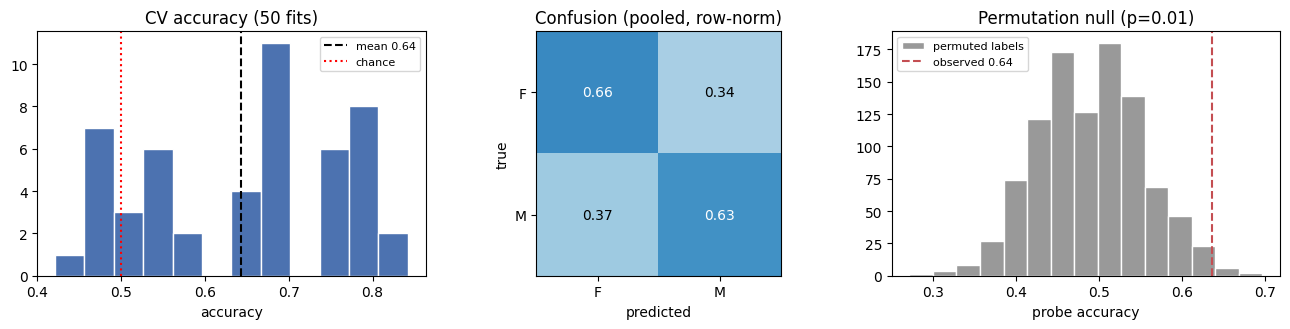
\includegraphics[width=0.7\linewidth]{13_classifier.png}
\caption{Proxy-task classifier performance (age group from frozen SFCN features).}
\label{fig:classifier}
\end{figure}

\subsection{Faithfulness}
ReX (M9) is in a different league from every other method: deletion AUC 0.141
([0.119, 0.165]) with high insertion AUC (0.755), meaning the voxels it flags genuinely
drive the output. Only the extremes are individually separable: ReX at the top, and LRP (M7)
and early-block Grad-CAM (M2) at the bottom. The five mid-ranked methods (Integrated
Gradients, Guided Backprop, SmoothGrad, Saliency, VarGrad) have heavily overlapping bootstrap
CIs and should be read as a tie, not a rank order. The paper's method (M1) is middling, and
early-block Grad-CAM (M2) is the worst of the nine (Table~\ref{tab:faith},
Fig.~\ref{fig:faith}).

\begin{table}[H]
\centering
\caption{Faithfulness. Deletion AUC (lower is better) with 95\% bootstrap CI; insertion AUC.}
\label{tab:faith}
\begin{tabular}{lccc}
\toprule
Method & Deletion AUC & 95\% CI & Insertion AUC \\
\midrule
M9 ReX & \textbf{0.141} & [0.119, 0.165] & 0.755 \\
M4 Integrated Gradients & 0.528 & [0.475, 0.584] & 0.512 \\
M8 Guided Backprop & 0.556 & [0.489, 0.624] & 0.742 \\
M5 SmoothGrad & 0.556 & [0.502, 0.609] & 0.537 \\
M3 Saliency & 0.568 & [0.518, 0.619] & 0.490 \\
M6 VarGrad & 0.580 & [0.531, 0.628] & 0.501 \\
M1 Grad-CAM (final) & 0.644 & [0.601, 0.687] & 0.501 \\
M7 LRP & 0.674 & [0.627, 0.720] & 0.598 \\
M2 Grad-CAM (early) & \textbf{0.777} & [0.730, 0.822] & 0.488 \\
\bottomrule
\end{tabular}
\end{table}

\begin{figure}[H]
\centering
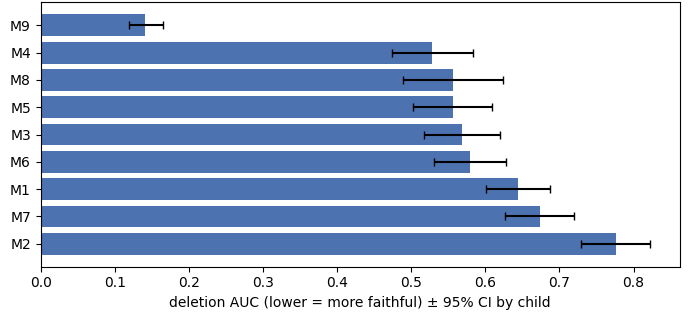
\includegraphics[width=0.85\linewidth]{08_faithfulness.png}
\caption{Deletion and insertion AUC across the nine methods.}
\label{fig:faith}
\end{figure}

\subsection{Randomized-weight sanity check}
Eight methods pass (low trained-vs-random correlation). \textbf{Integrated Gradients fails}
decisively ($r=0.73$): its map is almost unchanged when \emph{every} layer, backbone and head,
is reinitialized, so on this network it reflects image structure rather than learned content
(Table~\ref{tab:sanity}, Fig.~\ref{fig:sanity}). Because the randomization is complete rather
than head-only, this correlation cannot be an artifact of an unchanged frozen backbone: the
backbone is random too. This is the study's single most important caution, because IG is
widely used and visually convincing.

Guided Backprop (M8), our negative control, passes here ($r=0.168$), which is at first
surprising: \citet{adebayo2018} report it as largely invariant to model randomization and
therefore a method that typically \emph{fails} this check. Two things reconcile the
difference. First, the sanity verdict depends on architecture and implementation: Guided
Backprop's insensitivity was shown on 2D ImageNet CNNs with ReLU backprop overrides, and on a
frozen six-block 3D SFCN with a small trained head the trained-vs-random map is less
correlated. Second, passing the sanity check is necessary, not sufficient: M8 remains a poor
explanation on the metric that matters here, with a near-chance deletion AUC (0.556), so we do
not promote it on the strength of the sanity result alone.

\begin{table}[H]
\centering
\caption{Randomized-weight sanity check. Spearman correlation, trained vs.\ random model
(lower is better).}
\label{tab:sanity}
\begin{tabular}{lcl}
\toprule
Method & Spearman (trained vs.\ random) & Verdict \\
\midrule
M2 Grad-CAM (early) & $-0.242$ & PASS (model-dependent) \\
M9 ReX & 0.019 & PASS \\
M1 Grad-CAM (final) & 0.121 & PASS \\
M3 Saliency & 0.141 & PASS \\
M6 VarGrad & 0.153 & PASS \\
M8 Guided Backprop & 0.168 & PASS \\
M5 SmoothGrad & 0.172 & PASS \\
M7 LRP & 0.255 & PASS \\
\textbf{M4 Integrated Gradients} & \textbf{0.728} & \textbf{FAIL (input-driven)} \\
\bottomrule
\end{tabular}
\end{table}

\begin{figure}[H]
\centering
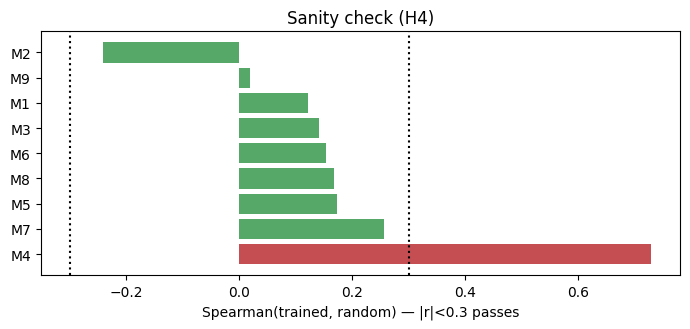
\includegraphics[width=0.85\linewidth]{09_sanity.png}
\caption{Sanity check: similarity between trained-model and random-model attributions.}
\label{fig:sanity}
\end{figure}

\subsection{Resolution}
The two methods that operate on the $5\times6\times5$ feature grid, final-block Grad-CAM (M1)
and ReX (M9), produce only about three large blobs each; in Fig.~\ref{fig:resolution} their
blob counts sit near zero against a scale dominated by the voxel-level methods, which fragment
into thousands of small blobs (SmoothGrad $\approx$19{,}000, Saliency $\approx$44{,}000). The
near-zero bars for M1 and M9 are therefore expected, not a plotting error: coarse grid-level
maps cannot have many blobs. This directly bears on the first open question about the original
analysis, namely that the explanation grid is coarser than many named structures.

\begin{figure}[H]
\centering
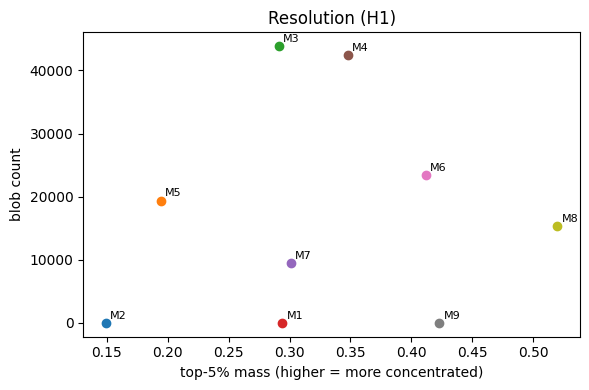
\includegraphics[width=0.85\linewidth]{12_resolution.png}
\caption{Resolution: top-5\% attribution mass and blob count per method. Grid-level methods
(M1 Grad-CAM final, M9 ReX) show $\approx$3 blobs, appearing near zero on the voxel-level
scale; this is inherent to the $5\times6\times5$ grid, not an artifact.}
\label{fig:resolution}
\end{figure}

\subsection{Cross-method agreement}
\begin{sloppypar}
Mean pairwise region-level Spearman correlation is only 0.36 (Fig.~\ref{fig:agreement}). The
gradient family (M3/M5/M6) agrees internally ($r$ up to 0.96), but the two Grad-CAM variants
are anti-correlated ($r=-0.61$), and ReX and LRP sit largely on their own.
Which ``important regions'' one reports depends heavily on the method chosen.
\end{sloppypar}

\begin{figure}[H]
\centering
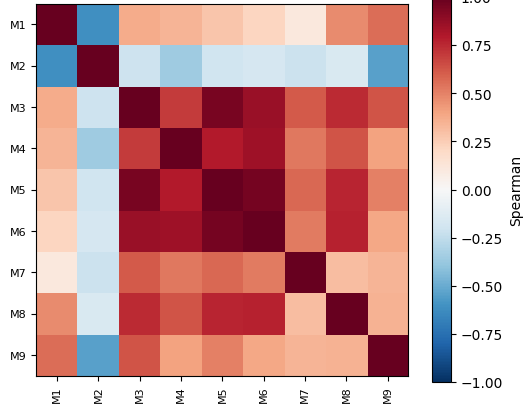
\includegraphics[width=0.7\linewidth]{11_agreement.png}
\caption{Pairwise cross-method agreement (region-level Spearman correlation).}
\label{fig:agreement}
\end{figure}

\subsection{Anatomical region test}
Under zero-fill masking, fifteen cortical regions survive Benjamini--Hochberg correction at
$q=0.05$ (Table~\ref{tab:regions}, Fig.~\ref{fig:regions}); the Lingual Gyrus carries by far
the largest effect. The result is fill-dependent: under the mean-intensity fill no region
survives correction (smallest raw $p=0.95$), so the regions below should be read as
significant for zero-region deletion specifically, not as a fill-robust anatomical claim. The
informative column is the effect size, not the FDR $p$: with a null of 200 random regions the
smallest attainable corrected $p$ is a floor (hence the repeated $0.017$), so the $p$ column
separates ``survives'' from ``does not'' but does not rank the regions. The full per-region
log (both fills, raw and corrected $p$) is released as
\texttt{results/region\_masking\_all\_pvalues.csv}.

\begin{table}[H]
\centering
\caption{The 15 cortical regions surviving BH-FDR $q=0.05$ under zero-fill masking. Effect is
the zero-fill masking effect size (probability drop); $n$ is region voxel count. The FDR $p$
is at the floor set by the 200-region null (see text), so effect size, not $p$, orders the
regions. No region survives under the mean-intensity fill.}
\label{tab:regions}
\small
\begin{tabular}{lrrr}
\toprule
Region & Effect & $n$ voxels & FDR $p$ \\
\midrule
Lingual Gyrus & 0.257 & 26{,}880 & 0.017 \\
Temporal Fusiform Cortex, posterior div. & 0.111 & 12{,}680 & 0.017 \\
Insular Cortex & 0.081 & 21{,}449 & 0.017 \\
Parahippocampal Gyrus, posterior div. & 0.069 & 5{,}698 & 0.017 \\
Inferior Temporal Gyrus, temporooccipital & 0.063 & 11{,}973 & 0.017 \\
Cingulate Gyrus, anterior div. & 0.059 & 20{,}844 & 0.017 \\
Parahippocampal Gyrus, anterior div. & 0.057 & 9{,}956 & 0.017 \\
Cingulate Gyrus, posterior div. & 0.057 & 19{,}228 & 0.017 \\
Occipital Fusiform Gyrus & 0.053 & 14{,}538 & 0.017 \\
Central Opercular Cortex & 0.044 & 14{,}953 & 0.017 \\
Parietal Operculum Cortex & 0.043 & 8{,}739 & 0.017 \\
Subcallosal Cortex & 0.039 & 9{,}021 & 0.017 \\
Frontal Operculum Cortex & 0.035 & 5{,}313 & 0.017 \\
Supramarginal Gyrus, posterior div. & 0.029 & 18{,}720 & 0.032 \\
Planum Temporale & 0.025 & 8{,}032 & 0.017 \\
\bottomrule
\end{tabular}
\end{table}

\begin{figure}[H]
\centering
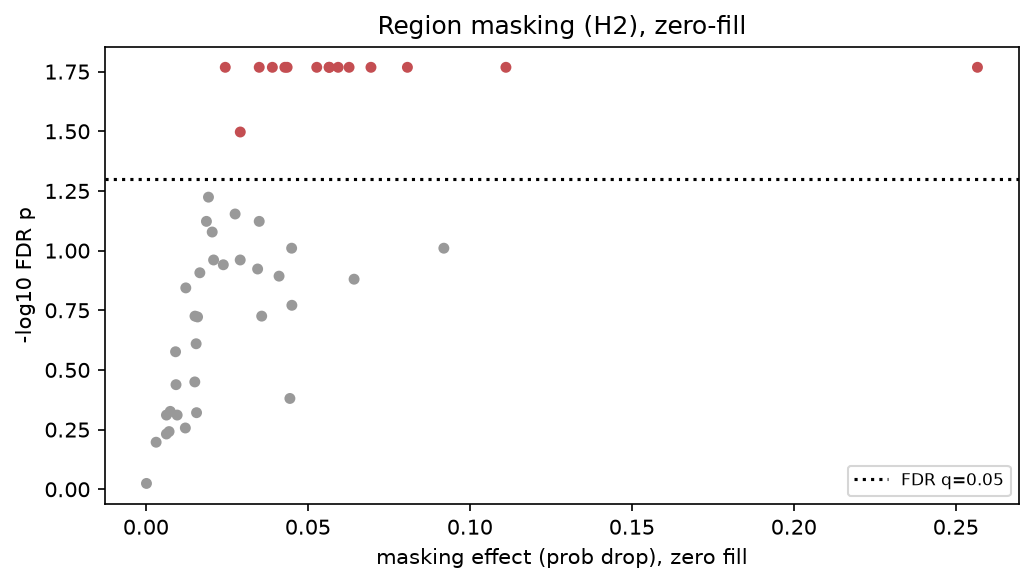
\includegraphics[width=0.85\linewidth]{10_region_masking.png}
\caption{Region masking test (zero fill) against a random-region null: zero-fill masking
effect size vs.\ $-\log_{10}$ FDR $p$. Red points survive BH-FDR $q=0.05$. The $x$-axis
matches the effect column of Table~\ref{tab:regions}.}
\label{fig:regions}
\end{figure}

\subsection{Layer probes and qualitative example}
Linear-probe accuracy was 0.624 from block~2 and 0.635 from block~6
(Fig.~\ref{fig:probes}): depth adds little for this task, and the proxy is almost as decodable
from an early block as from the final one. A representative scan across all nine methods
(Fig.~\ref{fig:example}) illustrates the resolution and agreement differences quantified above.

\begin{figure}[H]
\centering
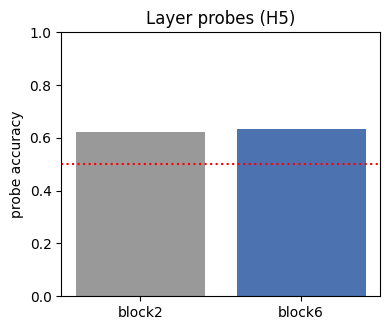
\includegraphics[width=0.6\linewidth]{14_layer_probes.png}
\caption{Linear-probe accuracy by feature block (block~2 vs.\ block~6).}
\label{fig:probes}
\end{figure}

\begin{figure}[H]
\centering
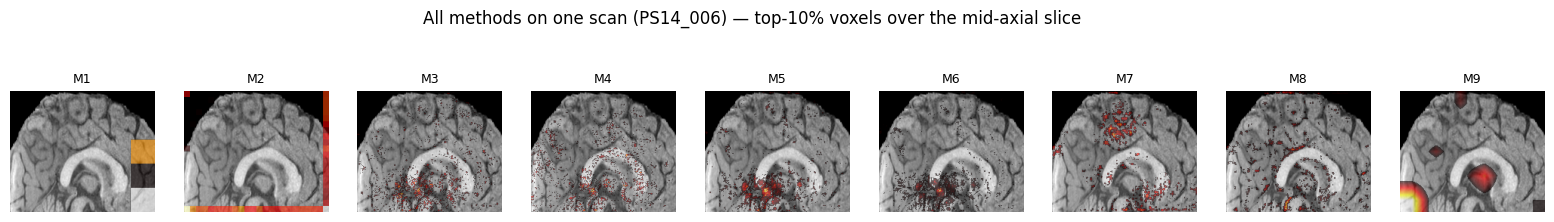
\includegraphics[width=\linewidth]{15_methods_example.png}
\caption{Qualitative attribution maps for one representative scan across all nine methods,
on matched slices. The resolution and agreement differences quantified in
Figs.~\ref{fig:resolution} and \ref{fig:agreement} are visible here.}
\label{fig:example}
\end{figure}

\section{Discussion}

\subsection{Pre-specified hypotheses}
Results are reported against the six hypotheses exactly as registered (OSF \texttt{jycnr}).

\textbf{H1} (Grad-CAM produces smoother, coarser maps than Integrated Gradients and SmoothGrad): \emph{supported}; early-block Grad-CAM is the most diffuse and carries the lowest top-5\% attribution mass, whereas the gradient methods are voxel-resolution and fragmented.

\textbf{H2} (large anatomical regions are more likely to survive correction than small named structures such as the pons and corpus callosum): \emph{not supported}; under the pre-specified mean-intensity fill no region survived BH-FDR ($q=0.05$), so the large-versus-small contrast could not be tested; a zero-fill sensitivity check yielded 15 surviving regions, confirming the region test is fill-dependent.

\textbf{H3} (Integrated Gradients and SmoothGrad correlate more with each other than either does with final-block Grad-CAM): \emph{supported descriptively}; mean pairwise region-level Spearman is 0.36, and the gradient family (including IG and SmoothGrad) agrees internally (up to $r=0.96$) while Grad-CAM sits apart. This is reported descriptively; no formal test of the difference between dependent correlations was pre-specified or run.

\textbf{H4} (for at least one method, randomized-weight maps differ from trained-weight maps): \emph{supported}; most methods change substantially under weight randomization; Integrated Gradients is the lone weak case, retaining the highest trained-versus-random similarity ($r=0.73$).

\textbf{H5} (a block-6 linear probe beats a block-2 probe): \emph{marginally supported}; 0.635 vs.\ 0.624.

\textbf{H6} (age-group accuracy exceeds chance under a child-level label-permutation test): \emph{supported}; cross-validated accuracy 0.635, permutation $p=0.01$ (1{,}000 permutations), confirming a usable but modest proxy signal.

\subsection{Deviations and exploratory analyses}
The following are not part of the registered hypotheses and are reported as exploratory: (i) the count of regions surviving correction and its dependence on the masking fill, an elaboration of H2; (ii) whether age is independently decodable from the frozen features as a possible confound (Ridge $R^2=0.11$); and (iii) fine-tuning the SFCN, which was pre-specified as out of scope and not run. Choices made after inspecting results are flagged as exploratory here and in the project decision log.

\subsection{The six open questions about the original analysis}
\label{sec:open}
\begin{enumerate}[leftmargin=1.6em]
\item \textbf{Coarse explanation grid}, \emph{confirmed}: Grad-CAM resolves to a few blobs on
the $5\times6\times5$ grid, coarser than named structures.
\item \textbf{Single region tested}, \emph{a corrected multi-region test is feasible}: it
finds 15 regions under zero-fill masking (none under mean-fill). This is a
different test from the original white-matter-volume $t$-test, not a like-for-like correction
of it, so we draw no comparison of effect direction or magnitude with \citet{das2024}; the
point is only that a multi-region, FDR-controlled test can be run where a single region was.
\item \textbf{Site/recruitment confound}, \emph{not testable}: PAE scans are not public.
\item \textbf{Age confound}, \emph{partially testable}: age is weakly decodable from the frozen
features ($R^2=0.11$); a plausible confound worth controlling.
\item \textbf{Child-level leakage}, \emph{addressed by design}: one scan per child and
child-grouped CV.
\item \textbf{Scan count vs.\ child count}, \emph{a counting distinction, not an error}: the
public release is longitudinal and lists multiple visits per child, so a T1 count (the
release lists on the order of 279) is larger than the number of unique children (96). We note
this only to explain why our $n$ is child-level; it is not a claim that any prior count was
wrong.
\end{enumerate}

\subsection{What this means in practice}
Method choice materially changes the reported ``important regions.'' Three practices follow:
report occlusion-based faithfulness (deletion/insertion) rather than trusting a map's
appearance; run a randomized-weight sanity check and discard methods that fail it (here,
Integrated Gradients); and never report a single method's regions without a corrected
statistical test.

\section{Limitations}
\label{sec:limits}
$n=96$; a single proxy task; one cortical atlas; and no PAE data. The backbone weights are the
public UK~Biobank brain-age release of \citet{peng2021} \citep{sfcnweights}; we report the
checkpoint used rather than relying on an unverified source. The proxy head is weak
($\approx$64\% CV accuracy), and faithfulness and sanity verdicts are properties of the
model being explained: a stronger classifier could rank the methods differently, so the
rankings here should be read as holding for this modest-accuracy model, not as universal. At
$n=96$ the study is powered for medium-to-large region
effects; small effects may be inconclusive (H3 and H4 do not depend on effect size). Two tests
we did not run bound the interpretation. First, we measured cross-method \emph{agreement} but
not true map \emph{stability}: we did not quantify how a single method's map varies under small
input perturbations or across random seeds, so claims about reproducibility within a method are
out of scope. Second, our sanity check uses complete model randomization; we did not perform the
layer-by-layer cascading randomization of \citet{adebayo2018}, which would localize where in the
backbone a method's dependence breaks down. Crucially, this work validates an explanation
protocol on an age-group proxy in public controls. It says \emph{nothing} about alcohol exposure,
FASD, or the original paper's clinical regions, which require the private PAE data. The
deliverable is the method verdict, not the accuracy.

\section{Conclusion}
On a frozen pretrained SFCN, nine explanation methods gave sharply different accounts of what
the model uses. Occlusion-based ReX was the most faithful; Integrated Gradients failed a basic
sanity check; methods agreed only weakly; and a corrected masking test isolated 15 cortical
regions under zero-fill, though not under the mean-intensity fill. The practical message for
neuroimaging XAI is that attribution maps must be validated
for faithfulness, model-dependence, and anatomical significance, before any of them is
read as evidence about the brain.

\section*{Reproducibility}
Data: public Calgary Preschool controls (OSF fork \texttt{5kz2p}, CC-BY 4.0). Code, the
pre-specified plan, all figures, and the full per-region $p$-value log are in the project
repository: \url{https://github.com/HoussemDs/brain-xai-faithfulness-audit}. The full pipeline
ran on Kaggle (GPU T4~$\times$2, $\approx$5.8\,h).

\bibliographystyle{plainnat}
\bibliography{references}

\appendix
\section{Supplementary preprocessing figures}
\begin{figure}[H]
\centering
\begin{subfigure}{0.46\linewidth}
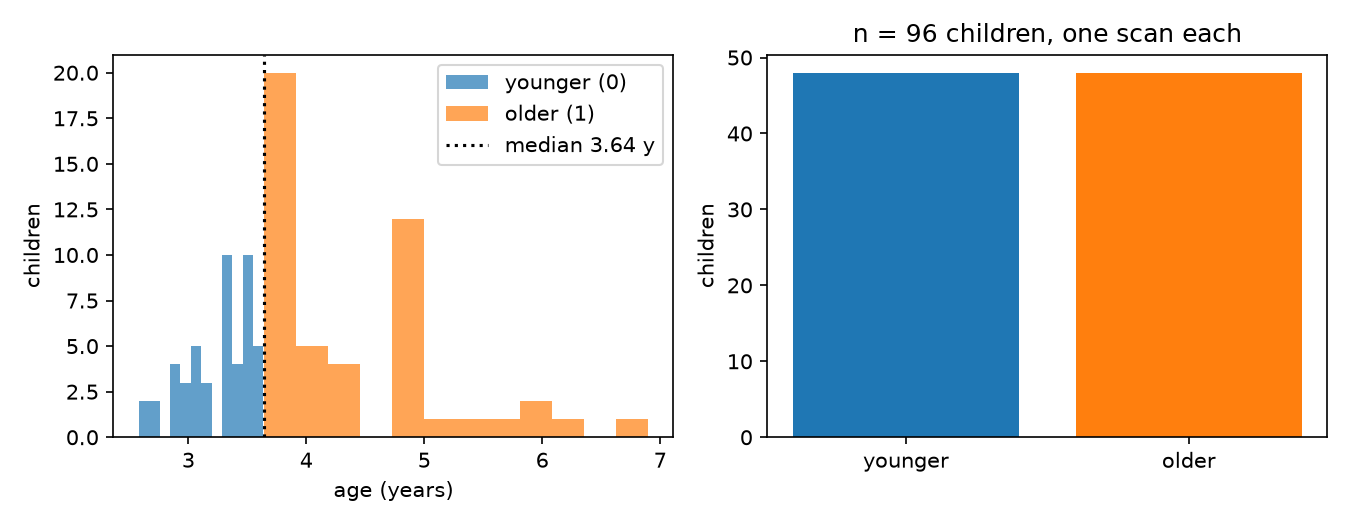
\includegraphics[width=\linewidth]{01_cohort_age_group.png}
\caption{Age-group split at the cohort median.}
\label{fig:cohort}
\end{subfigure}\hfill
\begin{subfigure}{0.46\linewidth}
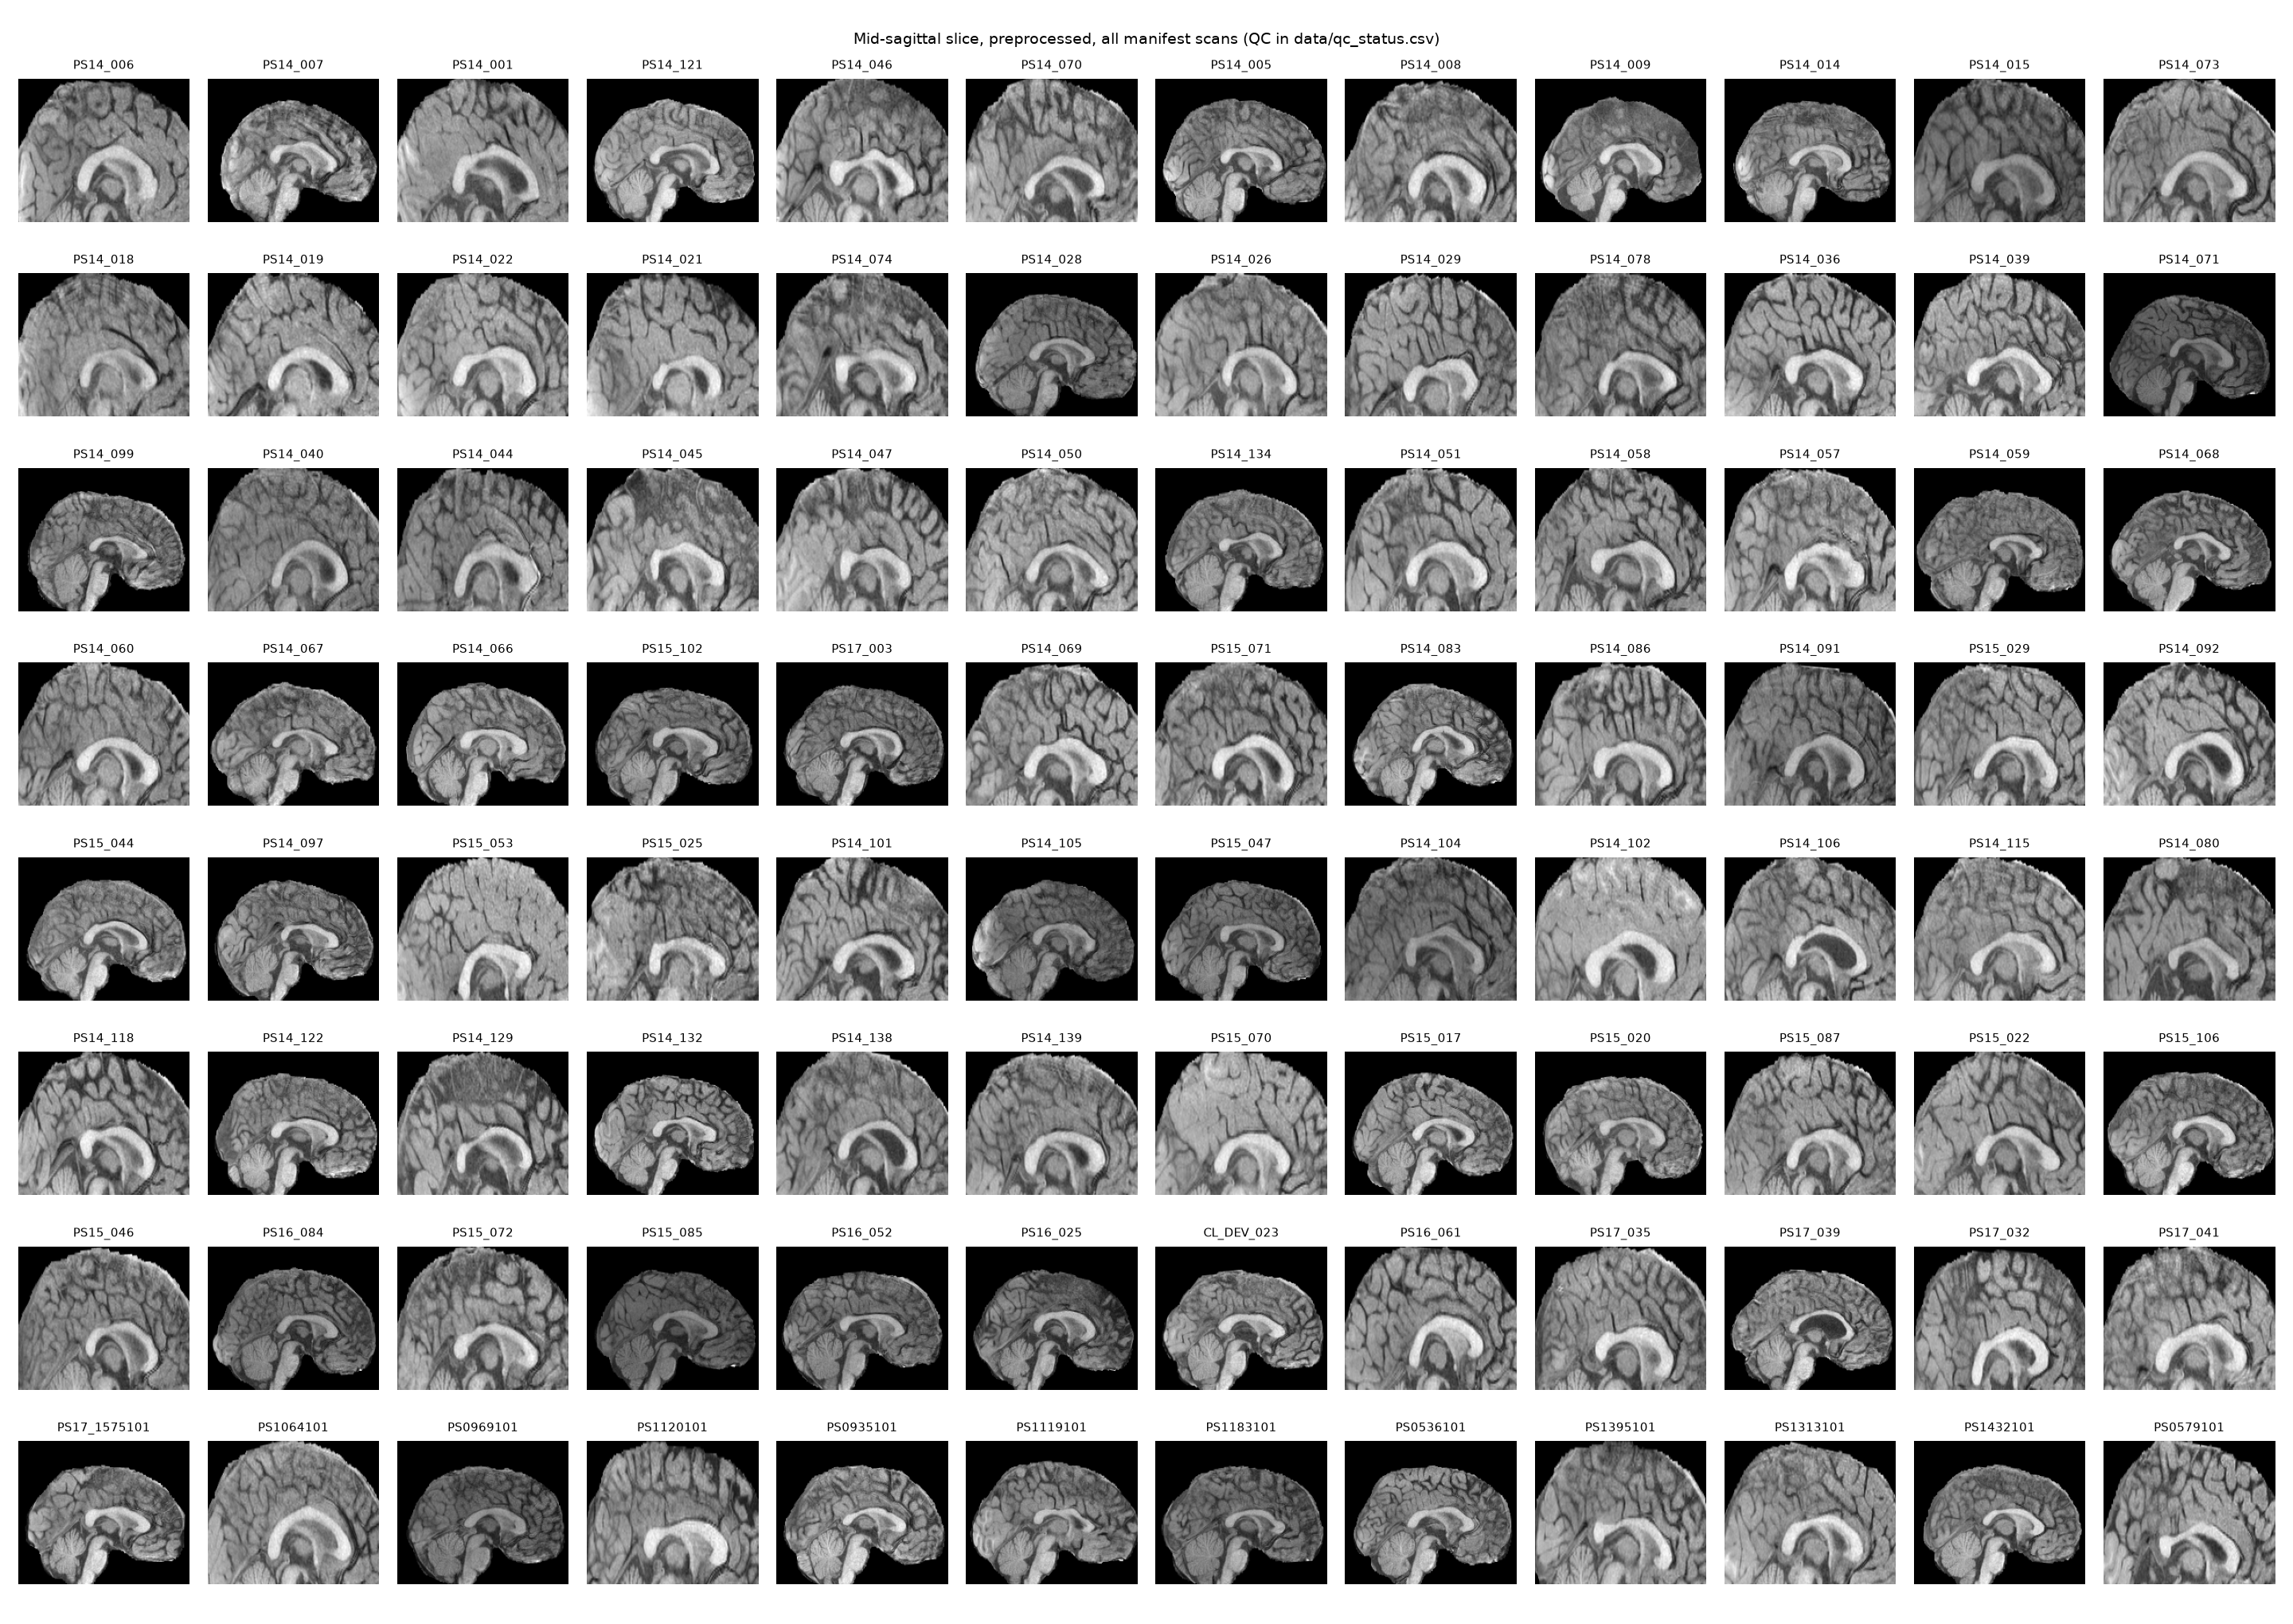
\includegraphics[width=\linewidth]{05_qc_contact_sheet.png}
\caption{QC contact sheet (all 96 scans).}
\label{fig:qc}
\end{subfigure}
\caption{Cohort and quality control.}
\end{figure}

\end{document}
